\documentclass{standalone}
\usepackage{tikz}
\usetikzlibrary{patterns, positioning}

\begin{document}
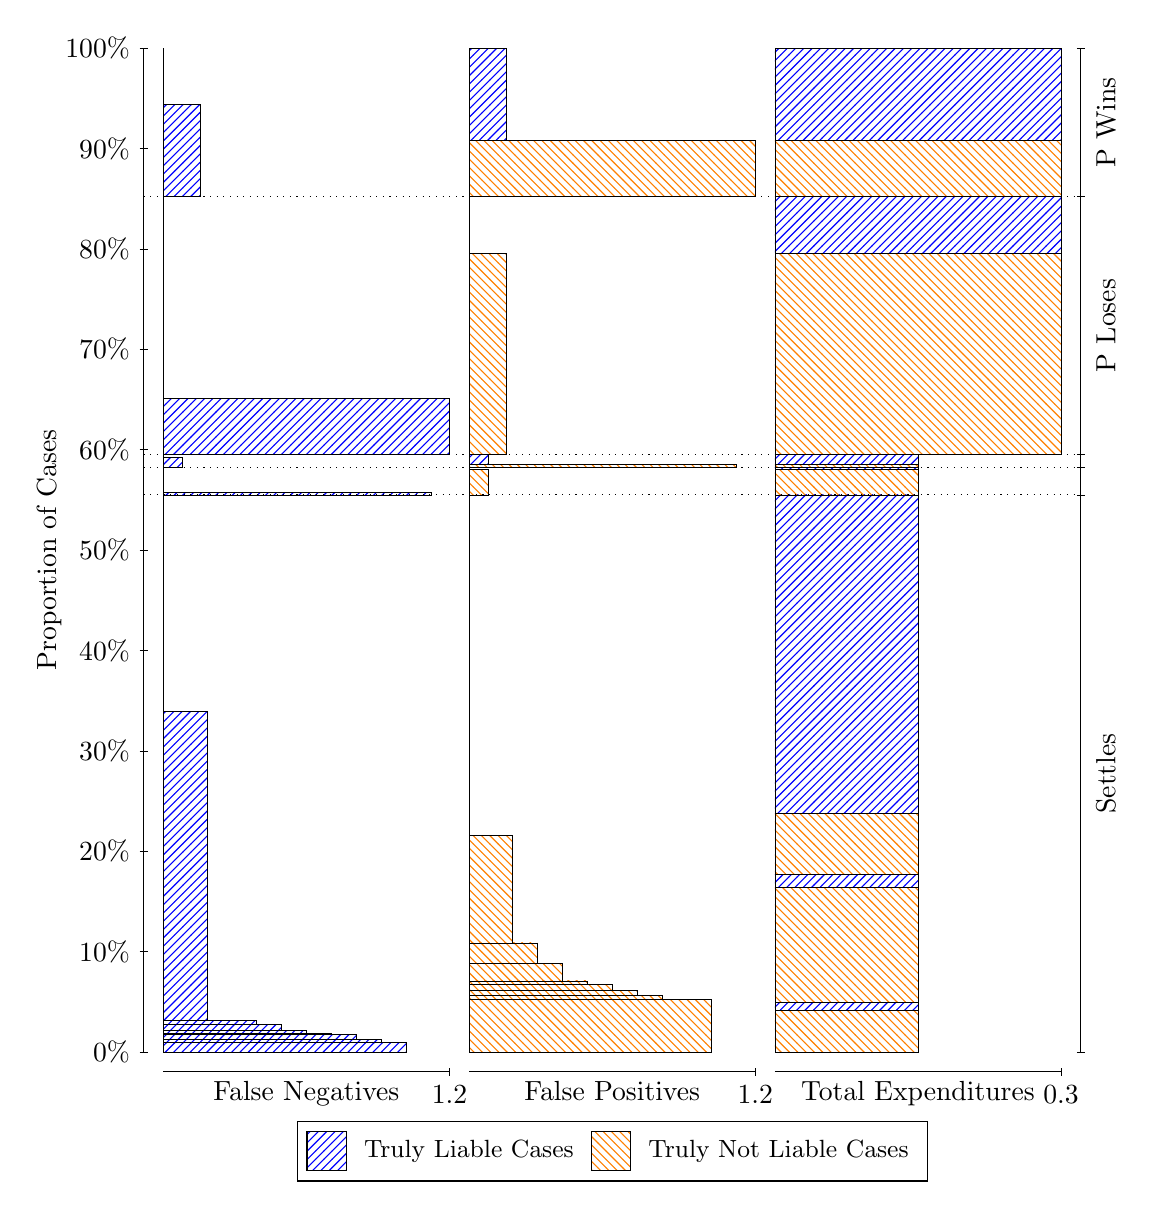
\begin{tikzpicture}
\draw[black, very thin] (1.5,1.75) -- (1.5,14.5);
\node[rotate=90, anchor=center] at (0.3, 8.125) {Proportion of Cases};
\draw[black, very thin] (1.45,1.75) -- (1.55,1.75);
\node[anchor=east] at (1.45, 1.75) {0\%};
\draw[black, very thin] (1.45,3.025) -- (1.55,3.025);
\node[anchor=east] at (1.45, 3.025) {10\%};
\draw[black, very thin] (1.45,4.3) -- (1.55,4.3);
\node[anchor=east] at (1.45, 4.3) {20\%};
\draw[black, very thin] (1.45,5.575) -- (1.55,5.575);
\node[anchor=east] at (1.45, 5.575) {30\%};
\draw[black, very thin] (1.45,6.85) -- (1.55,6.85);
\node[anchor=east] at (1.45, 6.85) {40\%};
\draw[black, very thin] (1.45,8.125) -- (1.55,8.125);
\node[anchor=east] at (1.45, 8.125) {50\%};
\draw[black, very thin] (1.45,9.4) -- (1.55,9.4);
\node[anchor=east] at (1.45, 9.4) {60\%};
\draw[black, very thin] (1.45,10.675) -- (1.55,10.675);
\node[anchor=east] at (1.45, 10.675) {70\%};
\draw[black, very thin] (1.45,11.95) -- (1.55,11.95);
\node[anchor=east] at (1.45, 11.95) {80\%};
\draw[black, very thin] (1.45,13.225) -- (1.55,13.225);
\node[anchor=east] at (1.45, 13.225) {90\%};
\draw[black, very thin] (1.45,14.5) -- (1.55,14.5);
\node[anchor=east] at (1.45, 14.5) {100\%};

\draw[black, very thin] (13.4,1.75) -- (13.4,14.5);
\draw[black, very thin] (13.35,1.75) -- (13.45,1.75);
\node[anchor=west] at (13.35, 1.75) {};
\draw[black, very thin] (13.35,8.8257) -- (13.45,8.8257);
\node[anchor=west] at (13.35, 8.8257) {};
\draw[black, very thin] (13.35,9.1751) -- (13.45,9.1751);
\node[anchor=west] at (13.35, 9.1751) {};
\draw[black, very thin] (13.35,9.3374) -- (13.45,9.3374);
\node[anchor=west] at (13.35, 9.3374) {};
\draw[black, very thin] (13.35,12.613) -- (13.45,12.613);
\node[anchor=west] at (13.35, 12.613) {};
\draw[black, very thin] (13.35,14.5) -- (13.45,14.5);
\node[anchor=west] at (13.35, 14.5) {};

\draw[black, very thin, pattern color=blue, pattern=north east lines] (1.75,1.75) rectangle (4.8304,1.8763);
\draw[black, very thin, pattern color=blue, pattern=north east lines] (1.75,1.8763) rectangle (4.5145,1.9136);
\draw[black, very thin, pattern color=blue, pattern=north east lines] (1.75,1.9136) rectangle (4.1986,1.9695);
\draw[black, very thin, pattern color=blue, pattern=north east lines] (1.75,1.9695) rectangle (3.8826,1.9872);
\draw[black, very thin, pattern color=blue, pattern=north east lines] (1.75,1.9872) rectangle (3.5667,2.0291);
\draw[black, very thin, pattern color=blue, pattern=north east lines] (1.75,2.0291) rectangle (3.2507,2.1021);
\draw[black, very thin, pattern color=blue, pattern=north east lines] (1.75,2.1021) rectangle (2.9348,2.1516);
\draw[black, very thin, pattern color=blue, pattern=north east lines] (1.75,2.1516) rectangle (2.6188,2.1524);
\draw[black, very thin, pattern color=blue, pattern=north east lines] (1.75,2.1524) rectangle (2.3029,6.0713);
\draw[black, very thin, pattern color=orange, pattern=north west lines] (1.75,6.0713) rectangle (1.75,8.8257);
\draw[black, very thin, pattern color=blue, pattern=north east lines] (1.75,8.8257) rectangle (5.1464,8.8565);
\draw[black, very thin, pattern color=orange, pattern=north west lines] (1.75,8.8565) rectangle (1.75,9.1751);
\draw[black, very thin, pattern color=blue, pattern=north east lines] (1.75,9.1751) rectangle (1.987,9.3045);
\draw[black, very thin, pattern color=orange, pattern=north west lines] (1.75,9.3045) rectangle (1.75,9.3374);
\draw[black, very thin, pattern color=blue, pattern=north east lines] (1.75,9.3374) rectangle (5.3833,10.054);
\draw[black, very thin, pattern color=orange, pattern=north west lines] (1.75,10.054) rectangle (1.75,12.613);
\draw[black, very thin, pattern color=blue, pattern=north east lines] (1.75,12.613) rectangle (2.2239,13.789);
\draw[black, very thin, pattern color=orange, pattern=north west lines] (1.75,13.789) rectangle (1.75,14.5);
\draw[black, very thin, pattern color=orange, pattern=north west lines] (5.6333,1.75) rectangle (8.7138,2.4212);
\draw[black, very thin, pattern color=orange, pattern=north west lines] (5.6333,2.4212) rectangle (8.3978,2.4227);
\draw[black, very thin, pattern color=orange, pattern=north west lines] (5.6333,2.4227) rectangle (8.0819,2.464);
\draw[black, very thin, pattern color=orange, pattern=north west lines] (5.6333,2.464) rectangle (7.7659,2.5281);
\draw[black, very thin, pattern color=orange, pattern=north west lines] (5.6333,2.5281) rectangle (7.45,2.6111);
\draw[black, very thin, pattern color=orange, pattern=north west lines] (5.6333,2.6111) rectangle (7.1341,2.6525);
\draw[black, very thin, pattern color=orange, pattern=north west lines] (5.6333,2.6525) rectangle (7.1341,2.6534);
\draw[black, very thin, pattern color=orange, pattern=north west lines] (5.6333,2.6534) rectangle (6.8181,2.8706);
\draw[black, very thin, pattern color=orange, pattern=north west lines] (5.6333,2.8706) rectangle (6.5022,3.135);
\draw[black, very thin, pattern color=orange, pattern=north west lines] (5.6333,3.135) rectangle (6.1862,4.5045);
\draw[black, very thin, pattern color=blue, pattern=north east lines] (5.6333,4.5045) rectangle (5.6333,8.8257);
\draw[black, very thin, pattern color=orange, pattern=north west lines] (5.6333,8.8257) rectangle (5.8703,9.1443);
\draw[black, very thin, pattern color=blue, pattern=north east lines] (5.6333,9.1443) rectangle (5.6333,9.1751);
\draw[black, very thin, pattern color=orange, pattern=north west lines] (5.6333,9.1751) rectangle (9.0297,9.208);
\draw[black, very thin, pattern color=blue, pattern=north east lines] (5.6333,9.208) rectangle (5.8703,9.3374);
\draw[black, very thin, pattern color=orange, pattern=north west lines] (5.6333,9.3374) rectangle (6.1072,11.896);
\draw[black, very thin, pattern color=blue, pattern=north east lines] (5.6333,11.896) rectangle (5.6333,12.613);
\draw[black, very thin, pattern color=orange, pattern=north west lines] (5.6333,12.613) rectangle (9.2667,13.323);
\draw[black, very thin, pattern color=blue, pattern=north east lines] (5.6333,13.323) rectangle (6.1072,14.5);
\draw[black, very thin, pattern color=orange, pattern=north west lines] (9.5167,1.75) rectangle (11.333,2.2738);
\draw[black, very thin, pattern color=blue, pattern=north east lines] (9.5167,2.2738) rectangle (11.333,2.3847);
\draw[black, very thin, pattern color=orange, pattern=north west lines] (9.5167,2.3847) rectangle (11.333,3.8373);
\draw[black, very thin, pattern color=blue, pattern=north east lines] (9.5167,3.8373) rectangle (11.333,4.0055);
\draw[black, very thin, pattern color=orange, pattern=north west lines] (9.5167,4.0055) rectangle (11.333,4.7836);
\draw[black, very thin, pattern color=blue, pattern=north east lines] (9.5167,4.7836) rectangle (11.333,8.8257);
\draw[black, very thin, pattern color=orange, pattern=north west lines] (9.5167,8.8257) rectangle (11.333,9.1443);
\draw[black, very thin, pattern color=blue, pattern=north east lines] (9.5167,9.1443) rectangle (11.333,9.1751);
\draw[black, very thin, pattern color=orange, pattern=north west lines] (9.5167,9.1751) rectangle (11.333,9.208);
\draw[black, very thin, pattern color=blue, pattern=north east lines] (9.5167,9.208) rectangle (11.333,9.3374);
\draw[black, very thin, pattern color=orange, pattern=north west lines] (9.5167,9.3374) rectangle (13.15,11.896);
\draw[black, very thin, pattern color=blue, pattern=north east lines] (9.5167,11.896) rectangle (13.15,12.613);
\draw[black, very thin, pattern color=orange, pattern=north west lines] (9.5167,12.613) rectangle (13.15,13.323);
\draw[black, very thin, pattern color=blue, pattern=north east lines] (9.5167,13.323) rectangle (13.15,14.5);
\draw[black, dotted] (1.5,8.8257) -- (13.4,8.8257);
\draw[black, dotted] (1.5,9.1751) -- (13.4,9.1751);
\draw[black, dotted] (1.5,9.3374) -- (13.4,9.3374);
\draw[black, dotted] (1.5,12.613) -- (13.4,12.613);
\draw[black, very thin] (1.75,1.5) -- (5.3833,1.5);
\node[anchor=north] at (3.5667, 1.5) {False Negatives};
\draw[black, very thin] (5.3833,1.45) -- (5.3833,1.55);
\node[anchor=north] at (5.3833, 1.45) {1.2};

\draw[black, very thin] (5.6333,1.5) -- (9.2667,1.5);
\node[anchor=north] at (7.45, 1.5) {False Positives};
\draw[black, very thin] (9.2667,1.45) -- (9.2667,1.55);
\node[anchor=north] at (9.2667, 1.45) {1.2};

\draw[black, very thin] (9.5167,1.5) -- (13.15,1.5);
\node[anchor=north] at (11.333, 1.5) {Total Expenditures};
\draw[black, very thin] (13.15,1.45) -- (13.15,1.55);
\node[anchor=north] at (13.15, 1.45) {0.3};

\node[black, centered, rotate=90] at (13.72, 5.2879) {Settles};


\node[black, centered, rotate=90] at (13.72, 10.975) {P Loses};
\node[black, centered, rotate=90] at (13.72, 13.556) {P Wins};

\draw (7.449999999999999,1.5) node[draw=none] (baseCoordinate) {};
\begin{scope}[align=center]
        \matrix[scale=0.5, draw=black, below=0.5cm of baseCoordinate, nodes={draw}, column sep=0.1cm]{
            \node[rectangle, draw, minimum width=0.5cm, minimum height=0.5cm, pattern=north east lines, pattern color=blue] {}; &
            \node[draw=none, font=\small] (B) {Truly Liable Cases}; &
            \node[rectangle, draw, minimum width=0.5cm, minimum height=0.5cm, pattern=north west lines, pattern color=orange] {}; &
            \node[draw=none, font=\small] (B) {Truly Not Liable Cases}; \\
            };
\end{scope}

\end{tikzpicture}
\end{document}